\documentclass{beamer}

\title{Raven Comparison Statistics}
\author{Josh Cogliati\\ (and this would not have happened without\\ Ivan Rinaldi and Cristian Rabiti.  \\Thanks also to Andrea Alfonsi and Diego Mandelli)}


\begin{document}

\begin{frame}
  \titlepage
\end{frame}

\begin{frame}
  \frametitle{Outline}
  \tableofcontents
\end{frame}

\section{Motivation}

\begin{frame}
  \frametitle{Why are we doing this?}
  We have codes that we need to compare to each other and to experiments.
\end{frame}

\begin{frame}
  \frametitle{Example}
  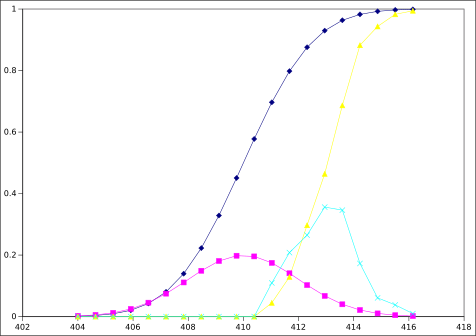
\includegraphics[height=6cm]{example}
\end{frame}

\section{Comparisons}

%cdf area difference
\begin{frame}
  \frametitle{CDF difference area}
  This calculates the difference in area between the two CDFs
  \begin{equation}
    cdf\_area\_difference = \int_{-\infty}^{\infty}{\|CDF_a(x)-CDF_b(x)\|dx}
  \end{equation}
  \begin{columns}
    \column{.5\textwidth}
    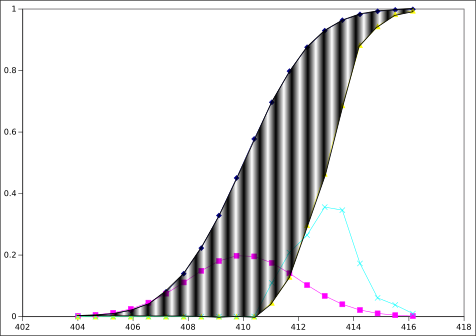
\includegraphics[height=3cm]{example_cdf_area}
    \column{.5\textwidth}
    Note that this area will have the same units as x.
  \end{columns}
\end{frame}

%common pdf area
\begin{frame}
  \frametitle{Common PDF area}
  This calculates the common area between the two PDFs.
  \begin{equation}
    pdf\_common\_area = \int_{-\infty}^{\infty}{\min(PDF_a(x),PDF_b(x))}dx
  \end{equation}
  \begin{columns}
    \column{.5\textwidth}
    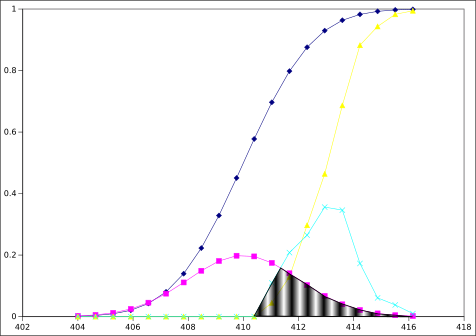
\includegraphics[height=3cm]{example_pdf_common}
    \column{.5\textwidth}
    This will range from 0\% to 100\%, with 100\% being a complete match.
  \end{columns}
\end{frame}


%difference between pdfs
\begin{frame}
  \frametitle{Difference between PDFs}
  This calculates a difference between the PDFs.
  \begin{equation}
    f_Z(z) = \int_{-\infty}^{\infty}f_X(x)f_Y(x-z)dx
  \end{equation}
  \begin{columns}
    \column{0.5\textwidth}
    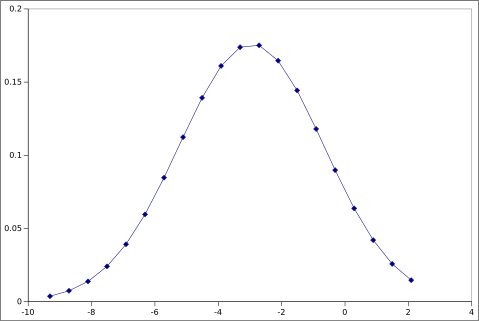
\includegraphics[height=3cm]{f_z}
    \column{0.5\textwidth}
    This generates a new pdf, with mean related
    to the average difference, and variance depending on a variety of
    factors.
  \end{columns}
\end{frame}

\begin{frame}
  \frametitle{Use of Differences between PDFs}
  This calculates the average:
  \begin{equation}
    \bar{z} = \int_{-\infty}^{\infty}{z f_Z(z)dz}
  \end{equation}
  This calculates the variance:
  \begin{equation}
    var = \int_{-\infty}^{\infty}{(z-\bar{z})^2 f_Z(z)dz}
  \end{equation}
\end{frame}

\section{Implementation}

%getting bins
\begin{frame}
  \frametitle{Getting the Numeric CDF and PDF}
  \begin{enumerate}
  \item Get the data and sort it
  \item Choose bins boundaries, and count the number of points in each bin
  \item Normalize the number of bins, and then calculate the running total to get the CDF
  \item Take the derivative of the CDF to get the PDF.
  \end{enumerate}
\end{frame}

%creating interpolation functions
\begin{frame}
  \frametitle{Interpolation functions}
  \begin{itemize}
  \item Using scipy's intererpolate.interp1d with the numeric data
  \item For the pdf, force the numbers outside the data to be zero
  \item For the cdf, force the numbers lower that the data to zero and higher to one
  \end{itemize}
\end{frame}

%integrating
\begin{frame}
  \frametitle{Integrating functions}
  \begin{itemize}
  \item Use Simpson method for calculating numbers
  \item For the pdfs and cdfs, use $-3\sigma+\mu$ to $3\sigma+\mu$ as
    the bounds (and the min and max of these if there are multiple
    ones)
  \item For the $f_Z$, the midpoint is $\mu_X-\mu_Y$ and the lower and
    upper bounds are $3\sigma_{max}$ away (where the largest $\sigma$
    is used).
  \end{itemize}
\end{frame}

\section{Future Directions}

\begin{frame}
  \frametitle{Future things to do}
  \begin{itemize}
  \item Multidimensional data
  \item Correlated data (input and output correlated)
  \item Flexibility for statistics (plugins or interfaces)
  \end{itemize}
\end{frame}

\section{Comments}

\begin{frame}
  \frametitle{Comments, complaints, concerns, contraindications, contributions \ldots ?}
\end{frame}

\end{document}
